%!TEX program=xelatex
\documentclass{article}

% Chinese font
\usepackage{xeCJK}
\usepackage{hyperref}

\setCJKmainfont{[kaiu.ttf]}
\setmainfont{[times new roman.ttf]}

\usepackage{colortbl}
\usepackage{xcolor}

\definecolor{LightGray}{gray}{0.8}
\newcolumntype{a}{>{\columncolor{LightGray}}c}
\newcolumntype{Y}{>{\centering\arraybackslash}X}

\usepackage{tabularx}
\usepackage{makecell}

\renewcommand*\contentsname{目錄}

\usepackage{graphicx}
\graphicspath{{./img/SDD}}

\usepackage{svg}
\svgpath{./img/SDD}

\usepackage{indentfirst}

\usepackage{minted}
\usepackage{caption}
\captionsetup{justification   = raggedright,
              singlelinecheck = false}

\usepackage{listings}
\lstset{basicstyle=\ttfamily,%
		breaklines=true,%
		breakatwhitespace=true,%
		keepspaces=true,%
		showspaces=false,%
		showstringspaces=false,%
		showtabs=false,%
		tabsize=2}

\newsavebox\jsoninputbox
\newsavebox\jsonoutputbox

\begin{document}
\begin{titlepage}
	\centering

	{\huge 海大教室借用平台}

	\vfill

	{\huge 設計文件}

	\vfill

	\begin{Large}
		\begin{center}
			\begin{tabular}{| a | c |}
				\hline
				專案名稱 & 海大教室借用平台               \\ \hline
				撰寫日期 & \today                 \\ \hline
				發展者  & \makecell{曾昱翔、林暐傑、陳鈺翔、 \\張銀軒、黃見弘} \\ \hline
			\end{tabular}
		\end{center}
	\end{Large}
\end{titlepage}


\addcontentsline{toc}{section}{版次變更紀錄}
\section*{版次變更紀錄}

\begin{tabularx}{\textwidth}{| c | X | X |}
	\rowcolor{LightGray}
	\hline
	版次    & 變更項目      & 變更日期       \\ \hline
	0.1   & 初版        & 2022/10/04 \\ \hline
	0.1.1 & 新增系統模型與架構 & 2022/11/28 \\ \hline
	0.1.2 & 新增介面需求與設計 & 2022/11/29 \\ \hline
	0.1.3 & 新增資料設計    & 2022/11/30 \\ \hline
	0.1.4 & 新增類別圖設計   & 2022/11/30 \\ \hline
	      &           &            \\ \hline
\end{tabularx}

\newpage

\begin{center}
	\tableofcontents
\end{center}

\newpage

\section[系統模型與架構(SYSTEM MODEL/SYSTEM ARCHITECTURE)]{系統模型與架構(System Model/System Architecture)}

\centerline{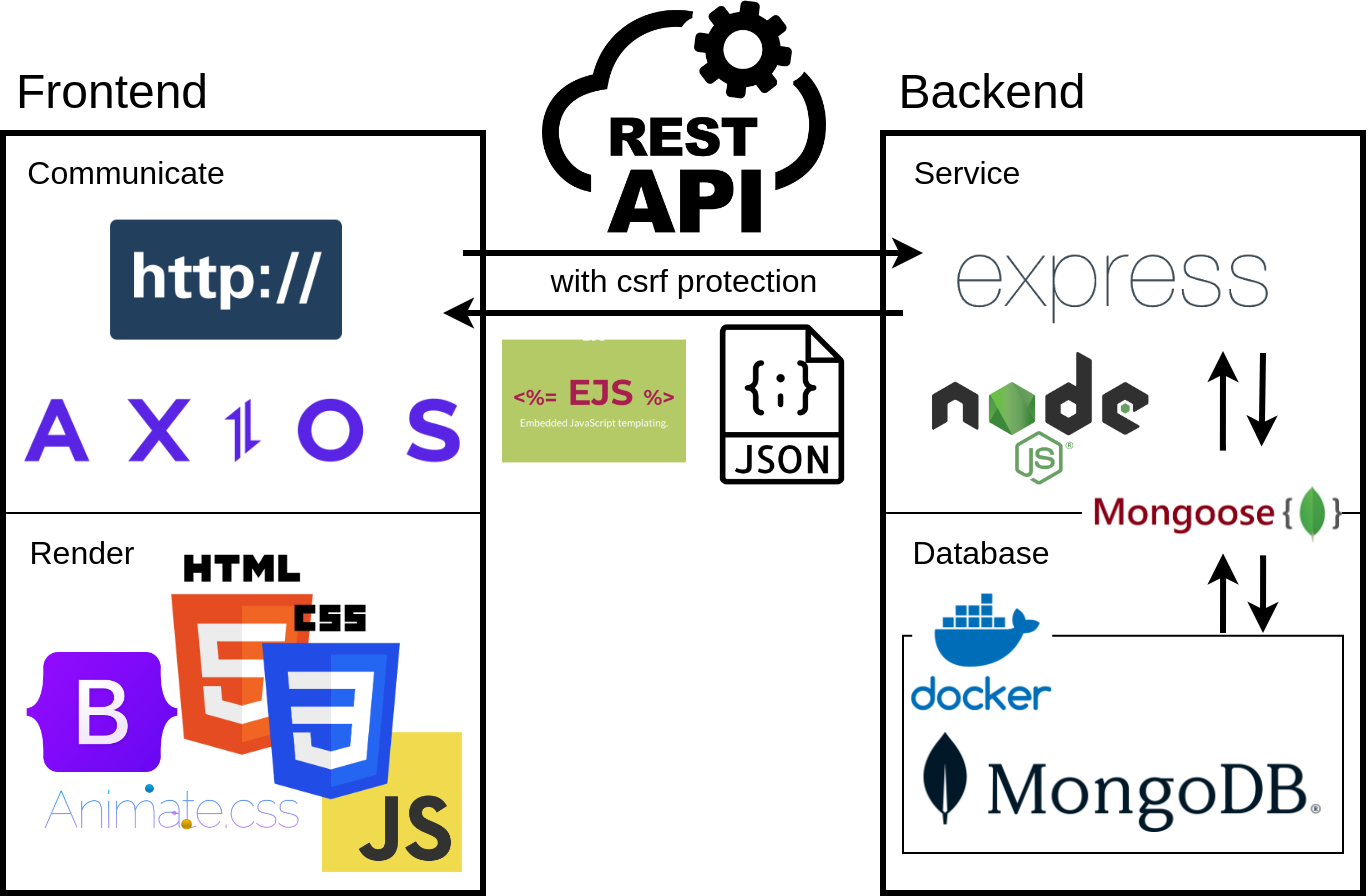
\includegraphics[width=\textwidth]{HighLevelArchitecture.png}}

\bigskip

前後端透過瀏覽器的 HTTP request 和 axios 提供的 request 方法與後端溝通,後端透過 express 提供的路由來處理前端的要求。

實際傳輸的方式包含了 RESTful API 和直接用 ejs render 後的結果當成網頁內容。

每個頁面透過瀏覽器發送的 request 來得到後端 ejs render 完的 HTML 內容,頁面中需要純前端處理的部分則以 axios 來傳送 request ,接收後端 render 完的 response 後直接操作 DOM 來改變頁面內容。

\subsection{後端架構}

後端架構主要分為兩個部分:後端伺服器和資料庫。

\subsubsection{後端伺服器}

伺服器為 Node.js express 搭配 ejs 來實作,主要負責處理前端的 request 並回傳給前端。

後端架構遵循 express-generator 產生出的 MVC 架構,將後端大致分為三個部分: routes、views 和 models 。

\subsubsection{資料庫}

透過 docker 來管理本地端的資料庫,使用的是 mongodb ,並在 express app 中以 mongoose ODM 來操作資料庫。

資料庫連線分為 \verb|/test| 和 \verb|/NTOUClassroomBorrowing| ,分別用來測試和正式使用。

\subsection{前端架構}

前端透過 Bootstrap 5 和基本的 HTML、CSS、JavaScript 來實作,主要負責處理使用者的操作並將結果傳送給後端。

部份動畫透過 animate.css 提供,純前端處理 request 的部份則以 axios 與後端溝通,收取 response 來更新頁面內容,或是彈出提示訊息。

\newpage

\section[介面需求與設計(INTERFACE REQUIREMENTS AND DESIGN)]{介面需求與設計(Interface Requirements and Design)}

\newcommand{\IRTable}[6]{
	\begin{tabularx}{0.95\textwidth}{|c|Y|Y|}
		\hline
		\rowcolor{LightGray} 介面名稱              & 介面提供者                & 介面使用者                 \\
		\rowcolor{LightGray} (Interface Name)  & (Interface Provider) & (Interface Consumer)  \\ \hline
		#1                                     & #2                   & #3                    \\ \hline
		\rowcolor{LightGray} 連結方式              & 輸入資料                 & 輸出資料                  \\
		\rowcolor{LightGray} (Connection Type) & (Input Data)         & (Output Data)         \\ \hline
		\texttt{#4}                            & \usebox\jsoninputbox & \usebox\jsonoutputbox \\ \hline
		\rowcolor{LightGray} \multicolumn{3}{|c|}{ URL }                                      \\ \hline
		\multicolumn{3}{|c|}{\texttt{#5}}                                                     \\ \hline
		\rowcolor{LightGray} \multicolumn{3}{|c|}{  介面描述 (Interface Description) }            \\ \hline
		\multicolumn{3}{|c|}{#6}                                                              \\ \hline
	\end{tabularx}
}

\subsection{帳號管理}

\begin{lrbox}{\jsoninputbox}
	\begin{lstlisting}
None
\end{lstlisting}
\end{lrbox}

\begin{lrbox}{\jsonoutputbox}
	\begin{lstlisting}
Plain HTML
\end{lstlisting}
\end{lrbox}

\IRTable{登入/註冊畫面}
{User 模組}
{登入/註冊頁面}
{HTTP GET}
{/users/session}
{回傳包含登入和註冊表單的頁面}

\bigskip

\begin{lrbox}{\jsoninputbox}
	\begin{lstlisting}[basicstyle=\tiny\ttfamily]
{
	"id": "10987654",
	"password": "password",
	"username": "name",
	"email": "email@mail.host",
	"phone": "0912345678"
}
\end{lstlisting}
\end{lrbox}

\begin{lrbox}{\jsonoutputbox}
	\makecell[l]{
		302 \texttt{/users/session} \\
		500 Internal Server Error
	}
\end{lrbox}

\IRTable{使用者註冊}
{User 模組}
{註冊表單}
{HTTP POST}
{/users/register}
{接收註冊表單,並將使用者資料存入資料庫}

\bigskip

\begin{lrbox}{\jsoninputbox}
	\begin{lstlisting}[basicstyle=\tiny\ttfamily]
{
	"id": "10987654",
	"password": "password",
}

\end{lstlisting}
\end{lrbox}

\begin{lrbox}{\jsonoutputbox}
	\makecell[l]{
		302 \texttt{/home} \\
		302 \texttt{/users/sesion}
	}
\end{lrbox}

\IRTable{使用者登入}
{User 模組}
{登入表單}
{HTTP POST}
{/users/login}
{接收登入表單,並將使用者資料存入 session}

\bigskip

\begin{lrbox}{\jsoninputbox}
	\begin{lstlisting}
{}
\end{lstlisting}
\end{lrbox}

\begin{lrbox}{\jsonoutputbox}
	302 \texttt{/users/sesion}
\end{lrbox}

\IRTable{使用者登出}
{User 模組}
{登出按鈕}
{HTTP POST}
{/users/logout}
{刪除 session 中之使用者資訊,並回到登入畫面}

\bigskip

\begin{lrbox}{\jsoninputbox}
	\begin{lstlisting}
None
\end{lstlisting}
\end{lrbox}

\begin{lrbox}{\jsonoutputbox}
	\begin{lstlisting}
Plain HTML
\end{lstlisting}
\end{lrbox}

\IRTable{待審使用者列表}
{Admin 模組}
{Admin/Account 頁面}
{HTTP GET}
{/admin/account}
{列出尚未審核之帳號}

\bigskip

\begin{lrbox}{\jsoninputbox}
	\begin{lstlisting}
None
\end{lstlisting}
\end{lrbox}

\begin{lrbox}{\jsonoutputbox}
	\begin{lstlisting}
Plain HTML
\end{lstlisting}
\end{lrbox}

\IRTable{查詢使用者資訊}
{Admin 模組}
{Admin/Account 頁面}
{HTTP GET}
{/admin/account/:id}
{查詢指定使用者之個人資訊}

\bigskip

\begin{lrbox}{\jsoninputbox}
	\begin{lstlisting}
{
	verified: true
}
\end{lstlisting}
\end{lrbox}

\begin{lrbox}{\jsonoutputbox}
	\makecell[l]{
		200 OK \\
		500 Internal Server Error
	}
\end{lrbox}

\IRTable{審核使用者}
{Admin 模組}
{Admin/Account 頁面}
{HTTP POST}
{/admin/account/:id}
{修改指定使用者審核狀態}

\pagebreak

\subsection{大樓、樓層與教室編輯}

\begin{lrbox}{\jsoninputbox}
	\begin{lstlisting}
None
\end{lstlisting}
\end{lrbox}

\begin{lrbox}{\jsonoutputbox}
	\begin{lstlisting}
	Plain HTML
\end{lstlisting}
\end{lrbox}

\IRTable{編輯頁面}
{Admin 模組}
{Admin/Classroom 頁面}
{HTTP GET}
{/admin/classroom}
{對大樓、樓層與教室進行編輯之主要操作頁面}

\bigskip

\begin{lrbox}{\jsoninputbox}
	\begin{lstlisting}[basicstyle=\footnotesize\ttfamily]
{ "name": "電機二館" }
\end{lstlisting}
\end{lrbox}

\begin{lrbox}{\jsonoutputbox}
	\begin{lstlisting}
200 OK
\end{lstlisting}
\end{lrbox}

\IRTable{新增大樓}
{Admin 模組}
{Admin/Classroom 頁面}
{HTTP POST}
{/admin/classroom/building}
{在資料庫中新增大樓}

\bigskip

\begin{lrbox}{\jsoninputbox}
	\begin{lstlisting}
None
\end{lstlisting}
\end{lrbox}

\begin{lrbox}{\jsonoutputbox}
	\begin{lstlisting}
200 OK
\end{lstlisting}
\end{lrbox}

\IRTable{刪除大樓}
{Admin 模組}
{Admin/Classroom 頁面}
{HTTP DELETE}
{/admin/classroom/building/:id}
{在資料庫中刪除大樓}

\bigskip

\begin{lrbox}{\jsoninputbox}
	\begin{lstlisting}[basicstyle=\tiny\ttfamily]
{
	"building": "電機二館",
	"floor": "一樓",
}
\end{lstlisting}
\end{lrbox}

\begin{lrbox}{\jsonoutputbox}
	\begin{lstlisting}
200 OK
\end{lstlisting}
\end{lrbox}

\IRTable{新增樓層}
{Admin 模組}
{Admin/Classroom 頁面}
{HTTP POST}
{/admin/classroom/floor}
{在指定的大樓中新增樓層}

\bigskip

\begin{lrbox}{\jsoninputbox}
	\begin{lstlisting}
None
\end{lstlisting}
\end{lrbox}

\begin{lrbox}{\jsonoutputbox}
	\begin{lstlisting}
200 OK
\end{lstlisting}
\end{lrbox}

\IRTable{刪除樓層}
{Admin 模組}
{Admin/Classroom 頁面}
{HTTP DELETE}
{/admin/classroom/building/:id/floor/:fid}
{刪除大樓中指定的樓層}

\bigskip

\begin{lrbox}{\jsoninputbox}
	\begin{lstlisting}
None
\end{lstlisting}
\end{lrbox}

\begin{lrbox}{\jsonoutputbox}
	\begin{lstlisting}
Plain HTML
\end{lstlisting}
\end{lrbox}

\IRTable{空教室表單}
{Admin 模組}
{Admin/Classroom 頁面}
{HTTP GET}
{/admin/classroom/empty}
{準備建立新教室時所需的表單}

\bigskip

\begin{lrbox}{\jsoninputbox}
	\begin{lstlisting}
None
\end{lstlisting}
\end{lrbox}

\begin{lrbox}{\jsonoutputbox}
	\begin{lstlisting}
Plain HTML
\end{lstlisting}
\end{lrbox}

\IRTable{教室資訊}
{Admin 模組}
{Admin/Classroom 頁面}
{HTTP GET}
{/admin/classroom/building/:id/floor/:fid/classroom/:cid}
{查詢指定教室的資訊}

\bigskip

\begin{lrbox}{\jsoninputbox}
	\begin{lstlisting}[basicstyle=\tiny\ttfamily]
{
	"building": "電機二館",
	"floor": "一樓",
	"name": "INS 103",
	"capacity": 30,
	"schedule":
		[
			[ null, lesson2, ... ],
			[ lesson1, null, ... ], ... 
		],
	"options": ["computer"]
}
\end{lstlisting}
\end{lrbox}

\begin{lrbox}{\jsonoutputbox}
	\begin{lstlisting}
200 OK
\end{lstlisting}
\end{lrbox}

\IRTable{建立新教室}
{Admin 模組}
{Admin/Classroom 頁面}
{HTTP POST}
{/admin/classroom}
{在指定的樓層中建立新教室}

\bigskip

\begin{lrbox}{\jsoninputbox}
	\begin{lstlisting}[basicstyle=\tiny\ttfamily]
{
	"building": "電機二館",
	"floor": "一樓",
	"name": "INS 103",
	"capacity": 30,
	"schedule":
		[
			[ null, lesson2, ... ],
			[ lesson1, null, ... ], ... 
		],
	"options": ["computer"]
}
\end{lstlisting}
\end{lrbox}

\begin{lrbox}{\jsonoutputbox}
	\begin{lstlisting}
200 OK
\end{lstlisting}
\end{lrbox}

\IRTable{更新教室}
{Admin 模組}
{Admin/Classroom 頁面}
{HTTP PUT}
{/admin/classroom/building/:id/floor/:fid/classroom/:cid}
{更新指定教室的資訊}

\bigskip

\begin{lrbox}{\jsoninputbox}
	\begin{lstlisting}
None
\end{lstlisting}
\end{lrbox}

\begin{lrbox}{\jsonoutputbox}
	\begin{lstlisting}
200 OK
\end{lstlisting}
\end{lrbox}

\IRTable{刪除教室}
{Admin 模組}
{Admin/Classroom 頁面}
{HTTP DELETE}
{/admin/classroom/building/:id/floor/:fid/classroom/:cid}
{刪除指定教室}

\pagebreak

\subsection{課程管理}

\begin{lrbox}{\jsoninputbox}
	\begin{lstlisting}
None
\end{lstlisting}
\end{lrbox}

\begin{lrbox}{\jsonoutputbox}
	\begin{lstlisting}
Plain HTML
\end{lstlisting}
\end{lrbox}

\IRTable{課程列表}
{Admin 模組}
{Admin/Lesson 頁面}
{HTTP GET}
{/admin/lesson}
{列出所有課程}

\bigskip

\begin{lrbox}{\jsoninputbox}
	\begin{lstlisting}[basicstyle=\tiny\ttfamily]
{
	"name": "課程A",
	"teacher": "王大明",
	"description": "課程A的說明"
}
\end{lstlisting}
\end{lrbox}

\begin{lrbox}{\jsonoutputbox}
	\begin{lstlisting}
200 OK
\end{lstlisting}
\end{lrbox}

\IRTable{新增課程}
{Admin 模組}
{Admin/Lesson 頁面}
{HTTP POST}
{/admin/lesson}
{新增一個課程於資料庫中}

\bigskip

\begin{lrbox}{\jsoninputbox}
	\begin{lstlisting}[basicstyle=\tiny\ttfamily]
{
	"name": "課程A",
	"teacher": "王大明",
	"description": "課程A的說明"
}
\end{lstlisting}
\end{lrbox}

\begin{lrbox}{\jsonoutputbox}
	\begin{lstlisting}
200 OK
\end{lstlisting}
\end{lrbox}

\IRTable{編輯課程}
{Admin 模組}
{Admin/Lesson 頁面}
{HTTP PUT}
{/admin/lesson/:id}
{編輯指定課程的資訊}

\bigskip

\begin{lrbox}{\jsoninputbox}
	\begin{lstlisting}
None
\end{lstlisting}
\end{lrbox}

\begin{lrbox}{\jsonoutputbox}
	\begin{lstlisting}
Plain HTML
\end{lstlisting}
\end{lrbox}

\IRTable{查詢課程}
{Admin 模組}
{Admin/Lesson 頁面}
{HTTP GET}
{/admin/lesson/:id}
{查詢指定課程的資訊}

\bigskip

\begin{lrbox}{\jsoninputbox}
	\begin{lstlisting}
None
\end{lstlisting}
\end{lrbox}

\begin{lrbox}{\jsonoutputbox}
	\begin{lstlisting}
200 OK
\end{lstlisting}
\end{lrbox}

\IRTable{刪除課程}
{Admin 模組}
{Admin/Lesson 頁面}
{HTTP DELETE}
{/admin/lesson/:id}
{刪除指定課程}

\bigskip

\begin{lrbox}{\jsoninputbox}
	\begin{lstlisting}
None
\end{lstlisting}
\end{lrbox}

\begin{lrbox}{\jsonoutputbox}
	\begin{lstlisting}
Plain HTML
\end{lstlisting}
\end{lrbox}

\IRTable{列出課表}
{Home 模組}
{Home 頁面}
{HTTP GET}
{/home/curriculum}
{列出當天課表}

\bigskip

\begin{lrbox}{\jsoninputbox}
	\begin{lstlisting}
None
\end{lstlisting}
\end{lrbox}

\begin{lrbox}{\jsonoutputbox}
	\begin{lstlisting}
Plain HTML
\end{lstlisting}
\end{lrbox}

\IRTable{列出課表}
{Home 模組}
{Home 頁面}
{HTTP GET}
{/home/curriculum/:date}
{列出指定日期的課表}

\bigskip

\begin{lrbox}{\jsoninputbox}
	\begin{lstlisting}
None
\end{lstlisting}
\end{lrbox}

\begin{lrbox}{\jsonoutputbox}
	\begin{lstlisting}
Plain HTML
\end{lstlisting}
\end{lrbox}

\IRTable{課程資訊}
{Home 模組}
{Home 頁面}
{HTTP GET}
{/home/lesson/:id}
{列出指定課程的資訊}

\newpage

\section[流程設計(PROCESS DESIGN)]{流程設計(Process Design)}

\newpage

\section[使用者畫面設計(USER INTERFACE DESIGN)]{使用者畫面設計(User Interface Design)}

\newpage

\section[資料設計(DATA DESIGN)]{資料設計(Data Design)}

\subsection{檔案結構}

\begin{itemize}
	\item \textbf{app.js}: 主程式
	\item \textbf{package.json}: 套件設定檔
	\item \textbf{public}: 靜態檔案
	\item \textbf{routes}: 路由
	\item \textbf{views}: 樣板
	\item \textbf{models}: 資料庫模組
	\item \textbf{middlewares}: 中介軟體
	\item \textbf{config}: 設定檔
	\item \textbf{bin}: 執行檔
	\item \textbf{node\_modules}: 套件
\end{itemize}

\pagebreak

\subsection{資料庫設計(Database Design)}

\begin{center}
	\captionof*{listing}{Building}
	\begin{minted}{js}
const buildingSchema = new mongoose.Schema({
  name: {
    type: String,
    required: true,
    unique: true,
    trim: true,
    minlength: 3,
  },
  floors: [
    {
      type: mongoose.Schema.Types.ObjectId,
      ref: "Floor",
    },
  ],
});
\end{minted}
\end{center}

\begin{center}
	\captionof*{listing}{Floor}
	\begin{minted}{js}
const floorSchema = new mongoose.Schema({
  name: {
    type: String,
    required: true,
  },
  building: {
    type: mongoose.Schema.Types.ObjectId,
    ref: "Building",
    required: true,
  },
  classrooms: [
    {
      type: mongoose.Schema.Types.ObjectId,
      ref: "Classroom",
    },
  ],
});
\end{minted}
\end{center}

\pagebreak

\begin{center}
	\captionof*{listing}{Classroom}
	\begin{minted}{js}
const classroomSchema = new mongoose.Schema({
  name: {
    type: String,
    required: true,
  },
  schedule: [
    [
      {
        type: mongoose.Schema.Types.ObjectId,
        ref: "Lesson",
      },
    ],
  ],
  capacity: {
    type: Number,
    required: true,
  },
  floor: {
    type: mongoose.Schema.Types.ObjectId,
    ref: "Floor",
    required: true,
  },
  options: [
    {
      type: String,
    },
  ],
});
\end{minted}
\end{center}

\pagebreak

\begin{center}
	\captionof*{listing}{Lesson}
	\begin{minted}{js}
const lessonSchema = new mongoose.Schema({
  name: {
    type: String,
    required: true,
  },
  teacher: {
    type: String,
    required: true,
  },
  borrowerID: {
    type: mongoose.Schema.Types.ObjectId,
    ref: "User",
  },
  description: {
    type: String,
  },
  fixed: {
    type: Boolean,
    default: false,
    required: true,
  },
});
\end{minted}
\end{center}

\pagebreak

\begin{center}
	\captionof*{listing}{User}
	\begin{minted}{js}
const userSchema = new mongoose.Schema({
  username: {
    type: String,
    required: true,
    unique: true,
    trim: true,
    minlength: 3,
  },
  password: { type: String, required: true, trim: true, minlength: 3 },
  email: {
    type: String,
    required: true,
    unique: true,
    trim: true,
    minlength: 3,
  },
  admin: { type: Boolean, required: true },
  id: { type: String, required: true, unique: true, trim: true, minlength: 3 },
  phone: {
    type: String,
    required: true,
    unique: true,
    trim: true,
    minlength: 3,
  },
  emailVerified: { type: Boolean, required: true },
  verified: { type: Boolean, required: true },
});
\end{minted}
\end{center}

\newpage

\section[類別圖設計(CLASS DIAGRAM DESIGN)]{類別圖設計(Class Diagram Design)}

\subsection{後端與資料庫 ODM}

\includesvg[inkscapelatex=false, width=\textwidth]{BackendClassDiagram.svg}

\bigskip

說明:程式主體為 \textbf{App} ,\textbf{App} 會使用 \textbf{Express} 建立伺服器,並使用 \textbf{Mongoose} 連接資料庫。
\textbf{App} 透過各個 \textbf{Router} 來處理使用者的請求,並使用 \textbf{Middleware(passport)} 來管理使用者登入狀態。
各個 \textbf{Router} 會依據需要使用相對應的 \textbf{Model} 來操作資料庫,並將結果傳回給使用者。

\pagebreak

\subsection{前端互動及資料傳輸}

\includesvg[inkscapelatex=false, width=\textwidth]{FrontendClassDiagram.svg}

說明:每個頁面皆包含 \textbf{Header} 和 \textbf{Topbar} ,分別為 \textbf{HTML} 的雜項設定和功能列。
其中多數函式皆在內部以純 \textbf{JavaScript} 實作(例如抓取元素資訊等),使用 \textbf{Axios} 來傳送請求至後端,並直接操作 \textbf{DOM} 來處理畫面的更新,達成前端的 \textbf{jQuery Free} 。

\newpage

\section[實作方案(IMPLEMENTATION LANGUAGE AND PLATFORM)]{實作方案(Implementation Language and Platform)}

\subsection{後端與資料庫}

後端採用 \textbf{Node.js} 的 \textbf{Express} 框架,並使用 \textbf{Mongoose} 來操作 \textbf{MongoDB} 資料庫。
使用者登入的部份由 \textbf{Node Package} 的 \textbf{Passport} 來建立 \textbf{Session} 。
\textbf{CSRF Protection} 也是使用 \textbf{Node Package} 提供的 \textbf{csurf} 套件來實作。
預計執行在 \textbf{x86\_64} 架構的 \textbf{Linux} 作業系統上,並使用 \textbf{Docker} 來建立 \textbf{MongoDB} 資料庫。
後續可能會使用 \textbf{Docker Compose} 來建立整個環境。

\subsection{前端}

前端採用 \textbf{Bootstrap 5} 框架配合基本的 \textbf{JavaScript} 和 \textbf{animate.css} ,並使用 \textbf{Axios} 來傳送請求至後端,以直接操作 \textbf{DOM} 的方式來處理畫面的更新。

\newpage

\section[設計議題(DESIGN ISSUE)]{設計議題(Design Issue)}

\end{document}